\documentclass[compress]{beamer}
\usetheme{sthlm}

%-=-=-=-=-=-=-=-=-=-=-=-=-=-=-=-=-=-=-=-=-=-=-=-=
%        LOADING BEAMER PACKAGES
%-=-=-=-=-=-=-=-=-=-=-=-=-=-=-=-=-=-=-=-=-=-=-=-=

\usepackage{
booktabs,
datetime,
dtk-logos,
graphicx,
multicol,
pgfplots,
ragged2e,
tabularx,
tikz,
wasysym,
multirow,
float,
caption,
subcaption
}

\pgfplotsset{compat=1.8}

\usepackage[utf8]{inputenc}
\usepackage[portuguese]{babel}
\usepackage[T1]{fontenc}
\usepackage{newpxtext,newpxmath}
\usepackage{listings}

\lstset{ %
language=[LaTeX]TeX,
basicstyle=\normalsize\ttfamily,
keywordstyle=,
numbers=left,
numberstyle=\tiny\ttfamily,
stepnumber=1,
showspaces=false,
showstringspaces=false,
showtabs=false,
breaklines=true,
frame=tb,
framerule=0.5pt,
tabsize=4,
framexleftmargin=0.5em,
framexrightmargin=0.5em,
xleftmargin=0.5em,
xrightmargin=0.5em
}



%-=-=-=-=-=-=-=-=-=-=-=-=-=-=-=-=-=-=-=-=-=-=-=-=
%        LOADING TIKZ LIBRARIES
%-=-=-=-=-=-=-=-=-=-=-=-=-=-=-=-=-=-=-=-=-=-=-=-=

\usetikzlibrary{
backgrounds,
mindmap
}

%-=-=-=-=-=-=-=-=-=-=-=-=-=-=-=-=-=-=-=-=-=-=-=-=
%        BEAMER OPTIONS
%-=-=-=-=-=-=-=-=-=-=-=-=-=-=-=-=-=-=-=-=-=-=-=-=

\setbeameroption{show notes}

%-=-=-=-=-=-=-=-=-=-=-=-=-=-=-=-=-=-=-=-=-=-=-=-=
%        BEAMER COMMANDS
%-=-=-=-=-=-=-=-=-=-=-=-=-=-=-=-=-=-=-=-=-=-=-=-=


%-=-=-=-=-=-=-=-=-=-=-=-=-=-=-=-=-=-=-=-=-=-=-=-=
%
%	PRESENTATION INFORMATION
%
%-=-=-=-=-=-=-=-=-=-=-=-=-=-=-=-=-=-=-=-=-=-=-=-=

\title{Comunicação por \\ mensagens - Sockets}
\subtitle{DCE540 - Computação Paralela e Distribuída}
%\date{\small{\jobname}}
\author{\texttt{Iago Carvalho}}
\institute{\texttt{Departamento de Ciência da Computação}}

\hypersetup{
pdfauthor = {Iago A. Carvalho},      
pdfsubject = {Computação Paralela e Distribuída},
pdfkeywords = {},  
pdfmoddate= {D:\pdfdate},          
pdfcreator = {WriteLaTeX}
}

\begin{document}

\begin{frame}
\titlepage

\end{frame}

%% --------------------------------------------------------

\begin{frame}{Defeitos do RPC}

Como vimos na aula passada, RPCs são mecanismos muito úteis

\vspace{1cm}

Entretanto, a necessidade de ambos os componentes (tanto o cliente quanto o servidor) estarem rodando é um grande problema

\vspace{1cm}

Além disso, o bloqueio do cliente (devido a comunicação síncrona) também não é desejável

\end{frame}


%% --------------------------------------------------------

\begin{frame}{Comunicação por mensagens}

Uma forma de contornar estes problemas é com a utilização de mensagens
\begin{itemize}
    \item Sockets TCP/IP
    \item Message Passing Interface (MPI)
    \item Fila de mensagens
    \item Message broker
    \item $\ldots$
\end{itemize}

\vspace{0.3cm}

Mensagens são transientes
\begin{itemize}
    \item Só existem enquanto a aplicação está sendo executada
\end{itemize}

\vspace{0.3cm}

Elas podem ser síncronas ou assíncronas
\end{frame}

%% --------------------------------------------------------

\begin{frame}{Sockets TCP/IP}

Um socket é um sistema para implementar troca de mensagens entre dois componentes na rede
\begin{itemize}
    \item Camada de transporte TCP/IP
    \item Padrão nos sistemas Unix e POSIX
    \item É uma interface padrão para comunicação entre processos
\end{itemize}

\vspace{0.75cm}

Um socket pode ser entendido como uma comunicação ponto-a-ponto entre dois componentes
\begin{itemize}
    \item Orientada a conexão (protocolo TCP)
    \item Utiliza IP para definir o endereço dos componentes
    \item Mensagem é enviada na rede
\end{itemize}
\end{frame}

%% --------------------------------------------------------

\begin{frame}{Operações de sockets TCP/IP}

Toda a comunicação por sockets é baseada em 8 diferentes operações (ou métodos)

\begin{enumerate}
    \item socket \textcolor{sthlmDarkBlue}{$\leftarrow$} cria uma nova conexão
    \item bind \textcolor{sthlmDarkBlue}{$\leftarrow$} atribui um endereço a um socket
    \item listen \textcolor{sthlmDarkBlue}{$\leftarrow$} "ouvir" a rede, esperando uma mensagem
    \item accept \textcolor{sthlmDarkBlue}{$\leftarrow$} aceita uma requisição de mensagem; bloqueio
    \item connect \textcolor{sthlmDarkBlue}{$\leftarrow$} tenta estabelecer uma conexão
    \item send \textcolor{sthlmDarkBlue}{$\leftarrow$} envia uma mensagem
    \item receive \textcolor{sthlmDarkBlue}{$\leftarrow$} recebe uma mensagem
    \item close \textcolor{sthlmDarkBlue}{$\leftarrow$} finaliza a conexão existente
\end{enumerate}

\end{frame}

%% --------------------------------------------------------

\begin{frame}{Comunicação por sockets}

\vspace{1cm}

\centering 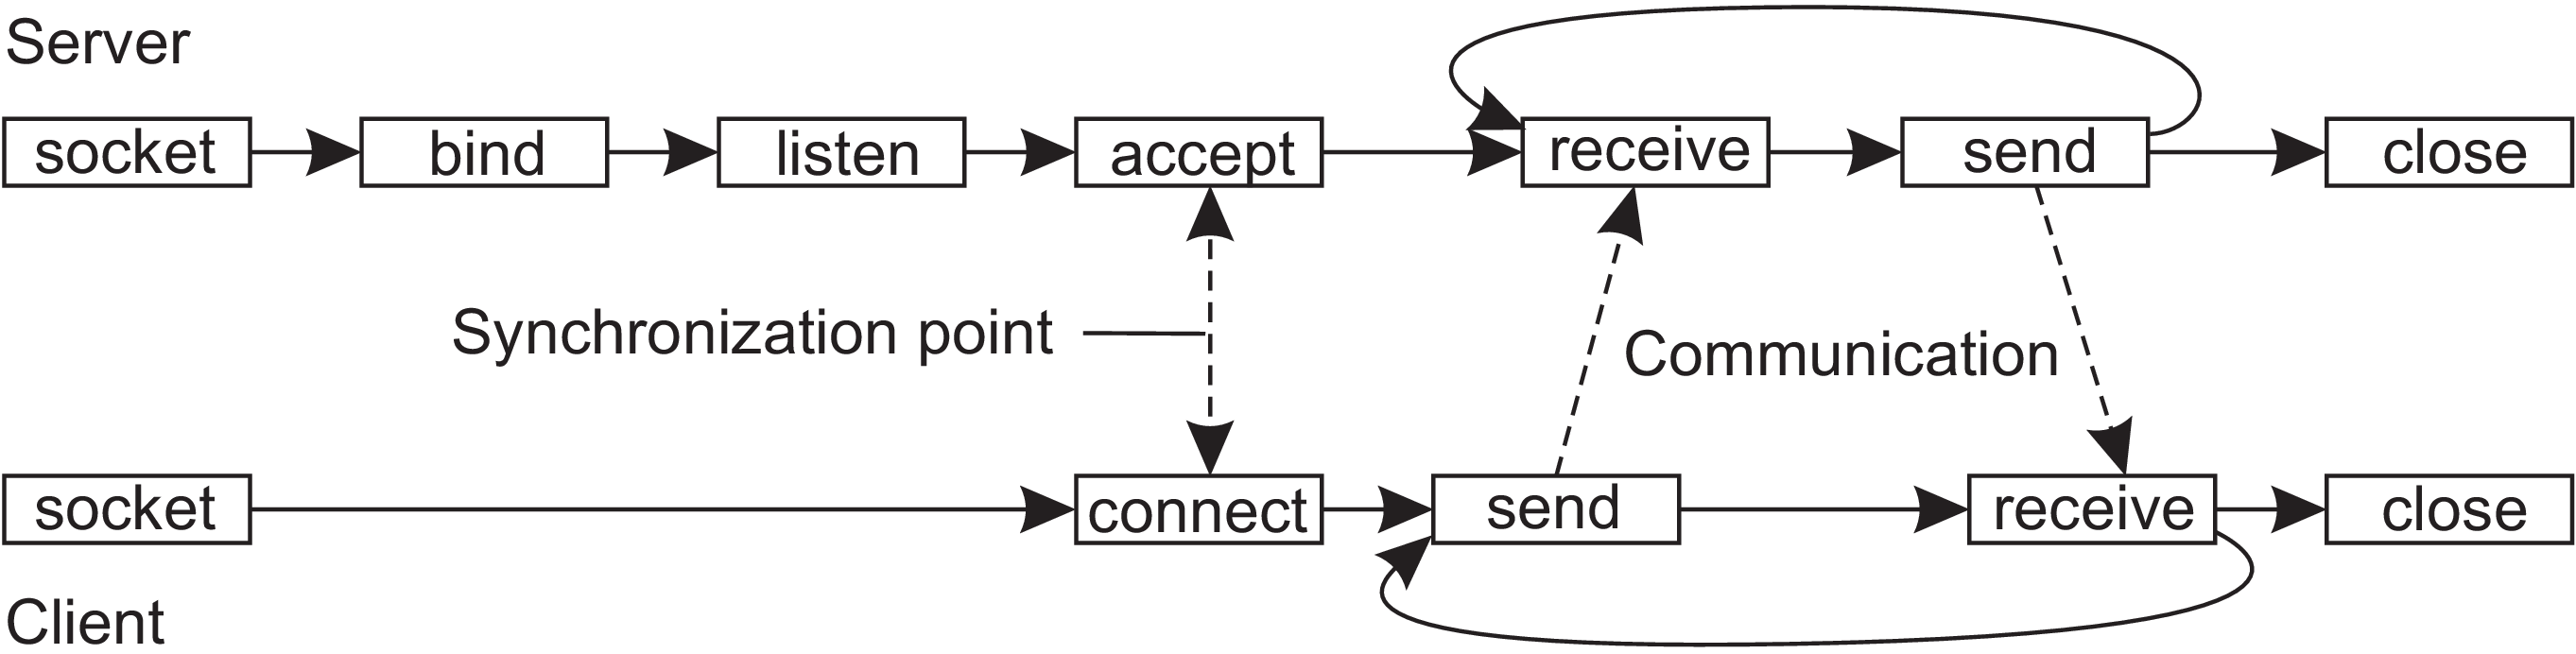
\includegraphics[width=\textwidth]{images/sockets.png}
\end{frame}

\end{document}
